\documentclass[twoside,english,notitlepage]{report}

\usepackage{geometry}
\usepackage{lipsum}
\usepackage[T1]{fontenc}
\usepackage{babel}
\usepackage{graphicx}
\usepackage{amsmath}
\usepackage{cite}
\usepackage{hyperref}
\usepackage{mathbbol}
\usepackage{multirow}
\usepackage{adjustbox}
\usepackage{multicol}

\geometry{
    a4paper,
    total={170mm,257mm},
    left=20mm,
    top=10mm,
}

\makeatletter
\def\@makechapterhead#1{%
    \vspace*{0\p@}%                                 % Insert 50pt (vertical) space
    {\parindent \z@ \raggedright \normalfont         % No paragraph indent, ragged right
    \ifnum \c@secnumdepth >\m@ne                   % If you should number chapters
        % \if@mainmatter                               % ... and you're in \mainmatter
        % \huge\bfseries \@chapapp\space \thechapter % huge, bold, Chapter + number – this is original
        \Huge\bfseries \thechapter.\space%
        % \par\nobreak                               % paragraph break without page break
        % \vskip 20\p@                               % Insert 20pt (vertical) space
    \fi
    \interlinepenalty\@M                           % Penalty
    \Huge \bfseries #1\par\nobreak                 % Huge, bold chapter title
    \vskip 30\p@                                   % Insert 40pt (vertical) space
}}
\makeatother


\title{CS424 – Group Project Report}
\author{
    Akeela Darryl Fattha\\
    \texttt{akeelaf.2022@scis.smu.edu.sg}
    \and
    Fadhel Erlangga Wibawanto\\
    \texttt{fadhelew.2022@scis.smu.edu.sg}
    \and
    Tan Zhi Rong\\
    \texttt{zhirong.tan.2022@scis.smu.edu.sg}
    \and
    Grace Angel Bisawan \\
    \texttt{gbisawan.2022@scis.smu.edu.sg}
    \and
    Lee Jia Heng\\
    \texttt{jiaheng.lee.2023@scis.smu.edu.sg}
}

\begin{document}
\date{}
\maketitle
\begin{abstract}
This report provides an overview of Cycle-Consistent Adversarial Networks (CycleGAN), a technique for unpaired image-to-image translation. We explore the architecture, key innovations, applications, and limitations of CycleGAN models in computer vision tasks.
\end{abstract}
\tableofcontents


\chapter{Task 1}

\section{Introduction}
We attempt to create a CyleGAN using novel and modern techniques to improve the performance of the model to convert cartoon faces to realistic faces, and vice-versa. We will be using improved blocks, various attention mechanisms and normalisation techniques in our generators, as well as additional loss functions to better guide the models to learn the mapping between the two domains. We opted not to use any augmentations to our images, and we use an image size of 256x256 as our input/output size. \\\\
With our enhancements, we achieved the following results:

\begin{table}[h]
    \centering
    \begin{tabular}{|l|c|c|c|c|}
    \hline
    \textbf{} & \textbf{FID} & \textbf{IS} & \textbf{GMS} & \textbf{Avg GMS} \\
    \cline{1-5}
    Raw to Cartoon     & 46.70193     & 2.41466 ± 0.24392   & 4.39783    & \multirow{2}{*}{3.85666} \\
    Cartoon to Raw     & 39.83461         & 3.62382 ± 0.23992        & 3.31548        &            \\
    \hline
    \end{tabular}
\end{table}

\subsection{Configuration \& Hyperparameters}
All optimisers used Adam with the following hyperparameters and loss weights:

\begin{multicols}{2}
    \begin{itemize}
        \item Random seed: 42
        \item Torch seed: 16109772023028774379
        \item n epochs: 100
        \item learning rate: 2e-4
        \item betas: (0.5, 0.999)
        \item $\lambda_{cyc}$: 10.0
        \item $\lambda_{id}$: 5.0
        \item $\lambda_{gan}$: 1.0
        \item $\lambda_{gp}$: 10.0
        \item $\lambda_{fm}$: 5.0
    \end{itemize}
\end{multicols}



\section{Architecture}
\subsection{Discriminator}
\paragraph{} Our discriminator uses a basic sequential architecture with convolutional layers that doubles in number of channels 3 times, from 64 to 512. Each convolution output is passed to a spectral norm layer, instance normalisation and a leaky relu activation function. We then branched into a Avg Pool into a FC layer for global classification and a PatchGAN block for local classification.

\begin{figure}[h]
    \centering
    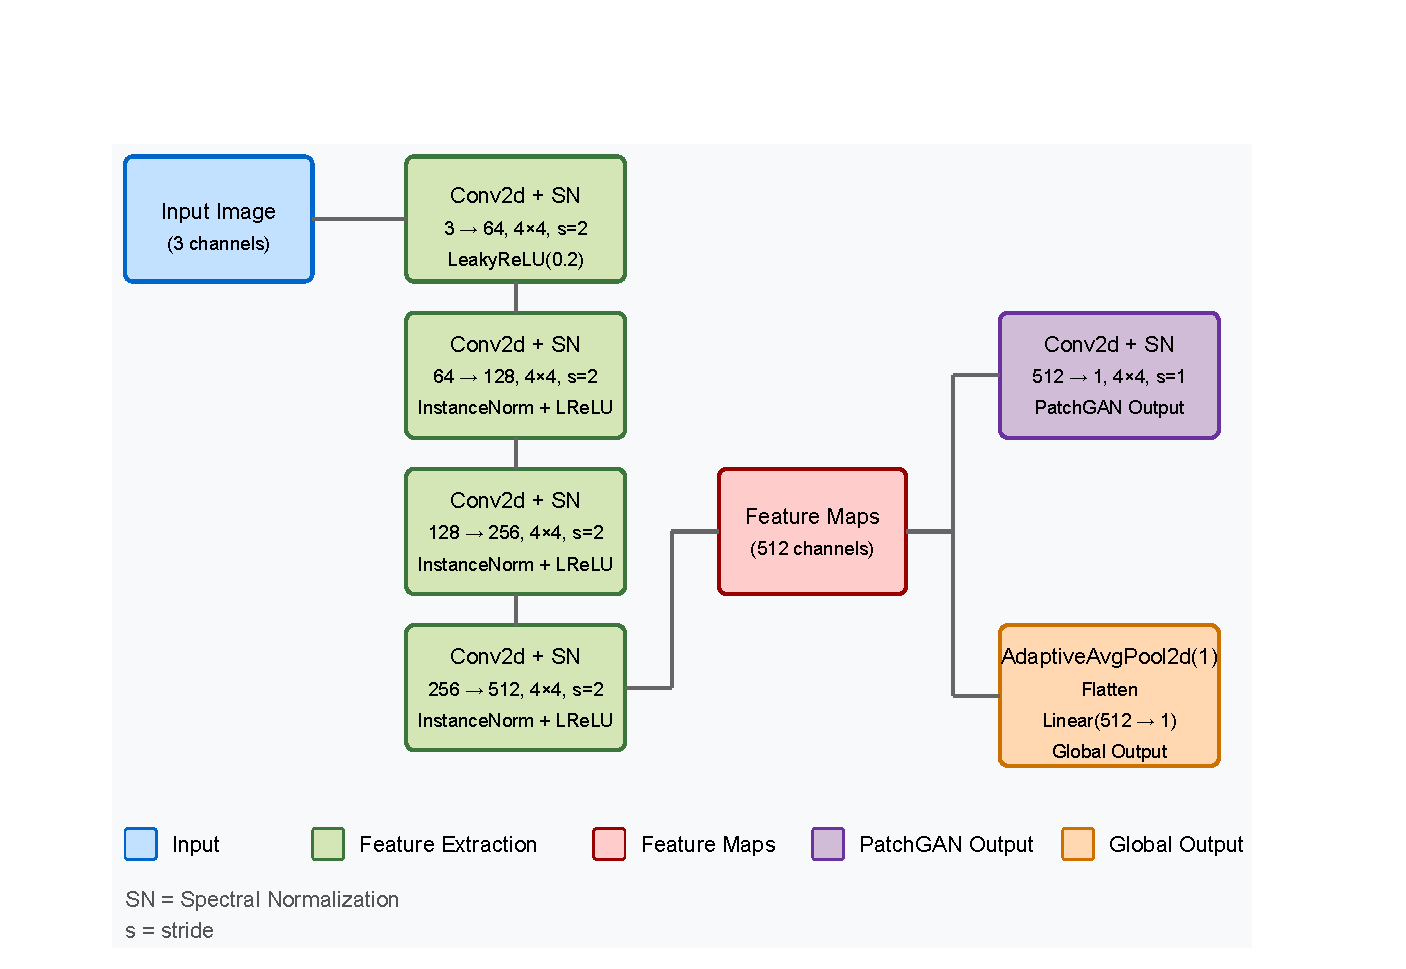
\includegraphics[width=0.8\textwidth]{task1/discriminator-architecture.pdf}
\end{figure}

\subsection{Generator}
\paragraph{} Our generator incorporates several modern attention mechanisms and architectural techniques including Convolutional Block Attention Module (CBAM), Squeeze-and-Excitation (SE) blocks, and Self-Attention mechanisms for improved feature representation, generating higher-quality images with better detail preservation, style consistency, and structural coherence.

\paragraph{} Some general key design choices include:
\begin{itemize}
    \item \textbf{Instance Normalization:} Used throughout the network instead of batch normalization, as it has been shown to produce better results for style transfer and image-to-image translation by normalizing each instance independently.

    \item \textbf{Reflection Padding:} Applied before convolutions to reduce boundary artifacts that can appear in generated images, particularly important for maintaining realistic edges.

    \item \textbf{Mixed Residual Blocks:} The strategic placement of different residual block types allows the network to benefit from complementary approaches to feature transformation:

    \begin{itemize}
        \item Style-modulated blocks provide explicit control over stylistic elements
        \item CBAM-enhanced blocks in the middle layers help focus on important features
        \item All blocks benefit from SE attention for channel recalibration
    \end{itemize}

    \item \textbf{Squeeze-and-Excitation Attention:} Used in Mixed Residual Blocks, it recalibrates channel-wise feature responses by explicitly modeling interdependencies between channels, allowing the network to selectively emphasize informative features.

    \item \textbf{Enhanced Self-Attention:} Positioned after the residual blocks, it helps ensure global coherence in the generated images by modeling long-range dependencies that convolutional operations cannot capture efficiently.

\end{itemize}

\paragraph{Improved Residual Block:} These blocks enhance the standard residual connection with both SE attention and conditional CBAM:

CBAM is applied to blocks 3-6, providing dual attention mechanisms:
\begin{itemize}
    \item \textbf{Channel Attention:} Models interdependencies between channels using both max and average pooling operations.
    \item \textbf{Spatial Attention:} Focuses on important spatial regions by creating attention maps from channel-wise statistics.
\end{itemize}

\paragraph{Style Modulated ResBlock:} Every third residual block employs style modulation through Adaptive Instance Normalization:
\begin{align}
    \text{AdaIN}(x) = \gamma \cdot \frac{x - \mu(x)}{\sigma(x)} + \beta
\end{align}

where $\gamma$ and $\beta$ are learnable style scale and bias parameters. This allows the network to better control stylistic elements in the generated images.

\subsubsection{Enhanced Self-Attention}
After the residual blocks, an enhanced self-attention module is applied:
\begin{align}
    \text{Attention}(Q, K, V) = \text{Softmax}\left(\frac{QK^T + P}{\sqrt{d_k}}\right)V
\end{align}

where $P$ represents the positional bias that emphasizes the central region. This self-attention mechanism allows the network to model long-range dependencies and coherence in the image, which is particularly valuable for maintaining structural integrity in facial regions.


\section{Data Preparation}
\subsection{Augmentations}
\paragraph{} We started with resizing images to 128x128, paired with a batch size of 16 before we hit a memory limit. We also applied no augmentations to the images, as a baseline to compare against later on when we add augmentations. 

\paragraph{} After adding various minor augmentations like affines, color jitters, flips, light gaussian blurs and posterising, we found that any combination of them resulted in worse metrics overall. From visual inspection, we found that the generated raw images were more noisy than without augmentations, which could contribute to the worse metrics. Furthermore, the generated cartoon images were a lot more flat than the target images, losing a lot more of the finer details and textures. Lastly, affines and any crops were clearly visible in the generated images when they otherwise should not be. 

\paragraph{} Thus, in both cases, we believe that adding the augmentations were encouraging the model to over-process the style conversions, which likely caused the reduction in metrics. Finally our best result was achieved with no augmentations, and upscaling the images to 256x256 with a batch size of 4. 

\vspace{20pt}
\begin{minipage}[t]{.47\textwidth}
    \centering
    \adjustbox{valign=t}{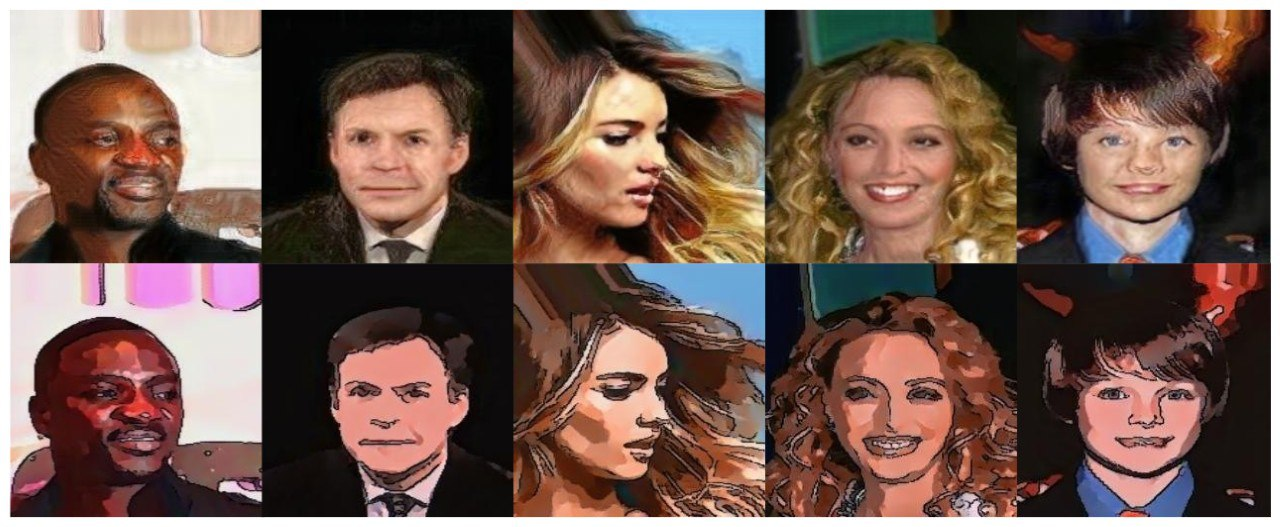
\includegraphics[scale=0.22]{task1/top1.jpg}}
    256x256 images Avg GMS: 3.85666
\end{minipage}
\begin{minipage}[t]{.47\textwidth}
    \centering
    \adjustbox{valign=t}{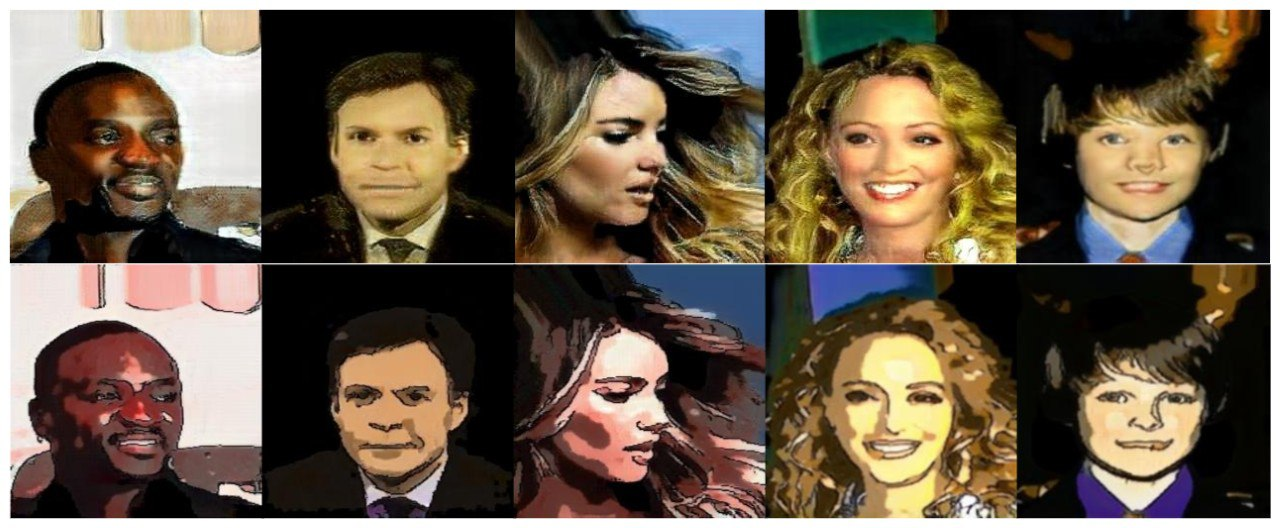
\includegraphics[scale=0.22]{task1/top2.jpg}}
    128x128 images Avg GMS: 4.47829
\end{minipage}

\subsection{Training/Validation}
\paragraph{} We worked with simple 99/1 split on training/validation data since we found that we needed as much data as possible for training the model to achieve our best results.

\paragraph{} We also made use of an "Image Pool" to help in training. This pool functions as a buffer to store previously generated images, which helps to reduce the risk of mode collapse where the Discriminator becomes too powerful, and prevents the Generator from learning anything new. The pool is updated with new generated fake images during training, and once the threshold is reached, we randomly sample from the available pool instead of using the latest generated image. 

\section{Loss Functions}

\subsection{Discriminator Losses}
We used a combination of loss functions beyond the standard adversarial loss to improve the performance of our discriminator. Our overall loss function for the discriminator is as follows:
\begin{equation}
    L_{D} = L_{GAN} + \lambda_{gp} L_{gp}
\end{equation}

\subsubsection{Gradient Penalty – $L_{gp}$}
We also use a gradient penalty, inspired from Wasserstein GAN (WGAN)\footnote{Arjovsky, M., Chintala, S., \& Bottou, L. (2017, July 17). Wasserstein Generative Adversarial networks. PMLR. \href{https://proceedings.mlr.press/v70/arjovsky17a.html}{https://proceedings.mlr.press/v70/arjovsky17a.html}} which improves stability of training, avoids problems like mode collapse with vanishing gradients, and ensures that the generator is always learning, even if it is not performing well enough to "beat" the discriminator.

\subsubsection{Relativistic – $L_{GAN}$}
We extend the typical adversarial loss by using a relativistic loss, which compares the logits of discriminating the real and fake images in a relative manner on a global scope with Binary Cross Entropy Loss. Furthermore, we took inspiration from PatchGAN\footnote{Isola, P., Zhu, J., Zhou, T., \& Efros, A. A. (2016). Image-to-Image Translation with Conditional Adversarial Networks. arXiv (Cornell University). \href{https://doi.org/10.48550/arxiv.1611.07004}{https://doi.org/10.48550/arxiv.1611.07004}} which whether the images is real or fake based on smaller patches, a local scope. Thus, we have another source of information for determining real or fake, which is computed with MSE loss. The equation for our relativistic loss for our "real" side is as follows, and the opposite will be applied for the "fake" side i.e. $D_{real} <=> D_{fake}, True <=> False$:
\begin{equation}
    L_{GAN} = 0.7 \cdot MSE(D_{real} - \bar{D}_{fake}, True)_{patch} + 0.3 \cdot BCE(D_{real} - \bar{D}_{fake}, True)_{global}
\end{equation}

\subsection{Generator Losses}
The generator also makes use of the \textbf{Relativistic} loss, which is an extension of the standard adversarial GAN loss. Our overall loss function for the generator is as follows:
\begin{equation}
    L_{G} = L_{GAN} + \lambda_{cyc} L_{cyc} + \lambda_{id} L_{id} + \lambda_{feat} L_{feat}
\end{equation}
\subsubsection{Cycle Consistency – $L_{cyc}$}
As we would like the fake images to be able revertible to its original image i.e. the pixels are identical, we maintain using L1 Loss for our Cycle Consistency.

\subsubsection{Identity – $L_{id}$}
Similarly, we also use L1 Loss for our Identity loss since images in the same domain should not be altered. 
\subsubsection{Feature – $L_{feat}$}
Another extension that we incorporated is the Feature Loss, which serves as a perceptual loss that compares the features of the generated image with the target image. Although traditionally used with pre-trained networks, we used the features extracted from the training discriminator instead. These features are compared using L1 loss, which helps to ensure that the generated images are perceptually similar to the target images. 

\chapter{Task 2}
\section{Introduction}



\subsection{Configuration}



\section{Architecture}
\subsection{Discriminator}
GANs consist of two networks: a generator that creates images and a discriminator that evaluates them. The two networks are trained adversarially, with the generator trying to fool the discriminator.

\subsection{Generator}
CycleGAN extends the GAN framework by using two generator-discriminator pairs, allowing translation between domains X and Y. The key innovation is the cycle-consistency loss, which ensures that translating an image to the target domain and back produces the original image.


\section{Data Preparation}
\subsection{Pre-Processing}
Used ChatGPT to generate a list of mapping of animal to pokemon variations


used a pretrained vgg16 to remove background for animals



\subsection{Training/Validation}
A simple 80/20 split on training data with validation



\section{Loss Functions}
Our overall loss functions for CycleGAN are as follows:


\begin{equation}
    L_{total} = L_{GAN} + \lambda_{cyc} L_{cyc} + \lambda_{id} L_{id} + \lambda_{edge} L_{edge} + \lambda_{color} L_{color}
\end{equation}

\subsection{Discriminator}
\subsubsection{Patch}

\subsubsection{Least Squares}

\subsection{Generator}

\subsubsection{Adversarial}
Use basic 

\subsubsection{Cycle Consistency}

\subsubsection{Identity}

\subsubsection{Edge Consistency}

\subsubsection{Color Consistency}

\subsection{Adaptive Loss Weighting}







\bibliographystyle{plain}
\bibliography{references}  % Create a references.bib file with your citations

\end{document}